\documentclass[titlepage]{article}
\usepackage[utf8]{inputenc}
\usepackage{graphicx,wrapfig}
\graphicspath{{images/}}
\usepackage{amsmath}

\usepackage{geometry}
 \geometry{
 a4paper,
 total={170mm,257mm},
 left=20mm,
 top=20mm,
 }

\title{B1-report-Nihaar}
\author{nihaar shah }
\date{December 2016}

\begin{document}

\maketitle
%Introduction to the document
\section{Introduction}
Resecting or calibrating a camera estimates the parameters of lens and image sensor of the camera. To estimate them you need to ha e 3D world coordinates and their corresponding 2D image points using multiple images of a calibration pattern. There may still be an error corresponding to the image distance between a projected point and a measured one. If we knew the true positions of the image points, we can minimize the minimum variance(?) cost between these image locations and predicted locations. This is called bundle –adjustment.
% Aim and motivation subsections of Intro
\subsection{Aim and Motivation}
To estimate and optimize the intrinsic parameters of a simplified ideal pinhole based model of a camera. This report attempts to test and explain the algorithms used and suggests further actions that can be done to achieve a commercial solution.
Knowledge of intrinsic parameters is very useful in finding real world distances of planar objects (given a single camera) if we know the position where the camera is mounted. Inversely if we know distances then we can estimate the camera location. Using stereo cameras we can estimate depth as well which is useful in visual odometry which has many applications in robotics.
% Specifications of the camera K matrix subsection of Intro
\subsection{Camera Model Specifications}
We have used an ideal pinhole simplification excluding effects of radial and tangential lens distortion. The 5 intrinsic parameters are chip width and height, focal length, effective width and height of pixel, skewness(\alpha) and principal point effects in x and y directions.
%
% The KMatrix equation 
\begin{equation} \label{KMatrix}
K=
  \begin{bmatrix}
  \alpha f & \gamma f & t_u \\ 
  0        & \beta f  & t_v \\ 
  0        &    0     &  1 
  \end{bmatrix}
\end{equation}
%Starting a new section
\section{Outline}
The main tasks and their corresponding equations are below:
% Simulation subsection of Outline
\subsection{Simulation}
In this project we are simulating the calibration object instead of using a real world calibration object to build our point correspondences between object and image. We use a known K-matrix to make these correspondences unlike in practice where the K matrix is unknown but the distances in the calibration object can be fed into the program to build the correspondences along with location of object in world coordinates. Thus, in this project we have functions to position the camera and object in world coordinates instead. A good test for these functions is to view a simulated cube as seen by the camera like in figure (1). Note the 4MP camera hence 2000 x 2000 dimensions of the image.
\begin{wrapfigure}{L}{4.5}
  \begin{center}
    \caption{Simulated cube in the camera's field of vision.}\label{wrap-fig:9}
    \includegraphics[width = 4.5cm, height=4.5cm]{SimulateCube.eps}
  \end{center}
  \caption{Birds}
\end{wrapfigure}
% Subsection on Estimation
\subsection{Initial Estimate}
% The object to image conversion equation 
\begin{equation}\label{uv-to-xy}
\begin{bmatrix}
  U\\ 
  V\\ 
  S 
  \end{bmatrix}
        = \textbf{K}
         \begin{bmatrix}
 \textbf{r1} & \textbf{r2} & \textbf{t}
         \end{bmatrix}
        \begin{bmatrix}
  x\\ 
  y\\ 
  1 
  \end{bmatrix}    
       =  \begin{bmatrix}
  h_{11}  & h_{12} & h_{13} \\ 
  h_{21}  & h_{22} & h_{23} \\ 
  h_{3_1}  & h_{32} & h_{33} 
  \end{bmatrix}
        \end{equation}
Equation 2 shows how we build point correspondences between object xy coordinates and image points (uv) from our checkerboard.  Equation 3 can be obtained by rearranging Equation 2.
%
% The object to image conversion equation 
\begin{equation}
    \label{Regressor}
  \begin{bmatrix}
  u\\ 
  v
  \end{bmatrix}
        = 
       \begin{bmatrix}
 x & y & 0 & 0 & 0 & -ux & -uy \\
 0 & 0 & 0 & x & y & 1 & -vx & -vy
  \end{bmatrix}
  \begin{bmatrix}
  h_{11}\\ 
    .\\
    .\\
  h_{32}
  \end{bmatrix}
 \implies \mathbf{p}_{j} = \mathbf{\Phi}_{j}  \mathbf{h}_{j}
      \end{equation}
% Build noisy image figure
\begin{wrapfigure}{R}{4.5}
  \begin{center}
    \label{wrap-fig:1}
    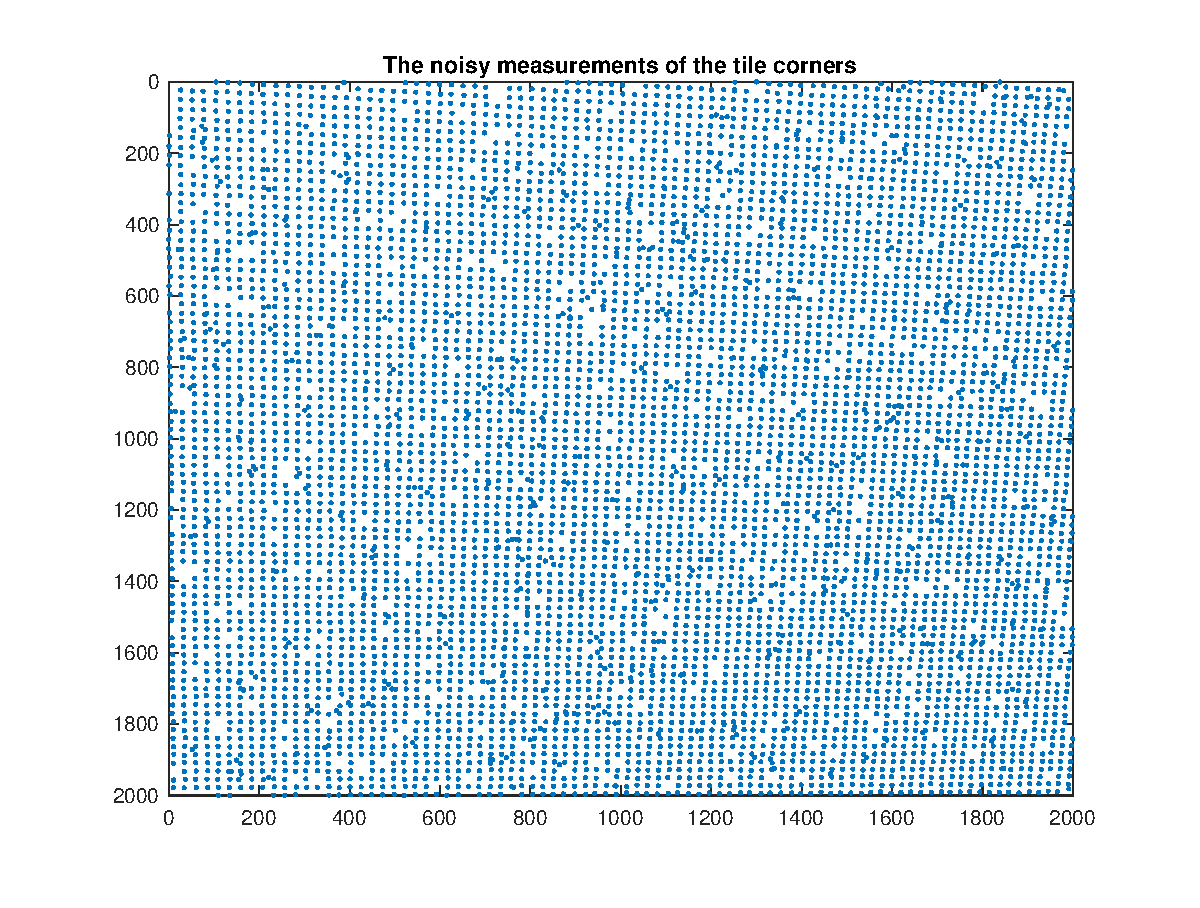
\includegraphics[width = 4.5cm, height=4.5cm]{GridImage.eps}
  \end{center}
  \caption{How the image of the grid appears on the camera sensor, noise included.}
\end{wrapfigure}
Using  n=4 known points we can solve the system using least squares minimization as shown in equation 4.
% The least squares minimum
\begin{equation}
    \label{Least Squares}
    \mathbf{H} = \lambda \mathbf{K} [\mathbf{r1} \mathbf{r2} \mathbf{t}] \implies \mathbf{K}^{-1} \mathbf{H} = \lambda [\mathbf{r1} \mathbf{r2} \mathbf{t}]\\
    min |\mathbf{\Phi} \mathbf{h} - \mathbf{p}|^2 \implies \mathbf{h} = [\mathbf{\Phi}^T \mathbf{\Phi}]^{-1} \mathbf{\Phi} \mathbf{p}
    \end{equation}
P and P are known. We use singular value decomposition svd to compute the inverse in 2q4 as that is computationally cheaper than using matlab inverse. This is called pseudo-inverse. (See discussion in approx. and assumption section 3).
Finally we want to estimate the K matrix from the Homography. We just found using 3 images of the same grid from different directions. We use the orthogonal property of the rotation matrix by pre-multiplying the Homography with the rotation to get Equation 5.
% K from H equation
\begin{equation}
    \label{K from H}
    \mathbf{H} = \lambda \mathbf{K} [\mathbf{r1} \mathbf{r2} \mathbf{t}] \implies \mathbf{K}^{-1} \mathbf{H} = \lambda [\mathbf{r1} \mathbf{r2} \mathbf{t}]\\
    \mathbf{H}^T \mathbf{K^{-1}}^{T} - \mathbf{K}^{-1} \mathbf{H} = \lambda^2 \mathbf{I}
    \end{equation}
This equation holds true for each image j and can be used to make a homogeneous equation of form Ax=0 to solve  \Phi = (K^-1)^T K^-1 again using svd and right singular vector of matrix \Phi associated with the smallest singular value. This is because for a homogeneous system any vector x in the null space of A is a solution hence any column of V whose corresponding singular value is zero is a solution. If we want a particular solution then we might want to pick the solution x with the smallest length |X|^2. We then obtain K from \Phi using cholesky factorization as we note that (K-^1)^T is an upper triangular matrix and K^-1 a lower triangular matrix.
% Starting subsection called Optimization
\subsection{Optimization}
So far we have gotten rid of outlier effects to an extent using RanSac. However Gaussian noise
(here in this project which was artificially added) still prevails. Using optimization of the least squares cost function we can tackle this Gaussian noise. Note that least squares form of cost function is an efficient way to eliminate noise but not outliers as it heavily penalizes Outliers. \\
Hence we use the two step approach- RanSac followed by least squares optimization. This is also a convex problem hence we should expect the global minimum and local minimum to be the same.
Decompose the Homography into the K-Matrix and positional parameters. Use this to predict the positions of points in the image using these transformation matrices and the current best camera matrix. The square of this minus the actual positions serves as our convex cost function.\\
We will use the Levenberg Marquardt algorithm to adjust parameters and decide when the minimum is reached. Steepest descent is a method to reach minimum by varying parameters \delta p along the steepest 'downhill' direction on the surface i.e. pointing along the negative gradient vector.
% Gradient descent equation
\begin{equation}
  \label{steepest_descent}
  \[ \delta \textbf{p} = -(\frac{\partial E}{\partial\mathbf{p}})^T = g_n\]
\end{equation}
%  
Newton steps method is based on taking a derivative of Taylor's expansion in N dimensions as shown in \ref{Newton_Step}   
% Newton step equation 
\begin{equation}
  \label{Newton_Step}
  \nabla (f(\textbf{x}+\delta\textbf{x}))=0 \implies g_n + H_n \delta p = 0\\
  \implies \delta{\mathbf{p}}=-\mathbf{H_n}^-1\mathbf{g_n}
\end{equation}
This gives the iterative update \mathbf{x_{n+1}}=\mathbf{x_n}-\mathbf{H_n}^-1 \mathbf{g}_n where \mathbf{H_n} is the Hessian matrix \frac{\partial^2 E}{\partial \mathbf{p}^2}. It is better to perform line search which ensures global cpnvergence hence we introduce the parameter \mu in \ref{Newton_Gradient}
% Newtonstep-Gradient descent  equation 
\begin{equation}
  \label{Newton_Gradient}
  \mathbf{x_{n+1}}=\mathbf{x_n}-\mu\mathbf{H_n}^-1 \mathbf{g}_n
\end{equation}
Combining \ref{Newton_Step} and \ref{Newton_Gradient} we get:
\begin{equation}
  \label{Final_Newton_Gradient}
  (\mathbf{H_n}+\mu\mathbf{I})\delta \mathbf{p}= -\mathbf{g}_n
\end{equation}
Therefore depending on \mu we can control between Newton steps and gradient descent.
% Start section on the overview of structure
\section{Overview of the Structure}
\subsection{Data Structure}
\subsection{Control Path}
\maketitle{RanSac flow}
\begin{wrapfigure}{R}{5.5cm}
  \label{Ransac_Flow}
  \caption{Flowchart for the Estimation task involving RansSac}\label{wrap-fig:1}
  \includegraphics[width = 5.5cm, height=14cm]{Ransac_flowchart.png}
\end{wrapfigure} 
RanSac is an alogorithm to eliminate outlier points - in this case points that are noisy in the calibration image. While estimating homography from the edges of the checkerboard we take 4 random points to build our regressor \Phi as seen in equation 4. To ensure these points are a true representation of the objects we perform Ransac.\\
As mentioned previously, in practice the computer automatically detects the edges of our checkerboard and build corresponding image coordinates given the dimensions of the board.
Then we choose 4 random points and build a homography. However how do we choose the 4 best points for this homography estimation? \\
We shall use RanSac so we can use that homography estimate which best agrees or is representative of maximum number of points on the checkerboard. The flowchart in figure 3 \ref{Ransac_Flow} shows this algorithm. Note that UV cordintes are the known points or true points. Using the homography, we multiply it with the xy object coordinates to obtain estimated U’V’. ranSac compares the difference between homography estimated U’V’ and true UV with a threshold MaxError  and populates a vector of points that satisfy this threshold as acceptable inliers. This set is called Best Consensus and then we construct our regressor of the over constrained system and use svd to find the least squares estimate of our final homography if the condition number is “good”. i.e. well conditioned system hence accurate inverse is possible. Once we have a good homography estimate it is straightforward to compute K using svd as mentioned earlier in section..
\title{Optimization flow}
The algorithm controls the search to move from steepest descent to newton steps depending on how well the last search performed. The feedback mechanism is that if the error has increased after changing the parameters along a certain direction then the weighting u is increased reducing the step size and causing the algorithm to just search downhill. If on the other hand the error has reduced that means we are closer to the minimum so we search in the neighborhood itself using Newton steps.
\begin{wrapfigure}{R}{5.5cm}
  \label{Optim_Flow}
  \caption{Flowchart for Optimization:the L-M algorithm}\label{wrap-fig:1}
  \includegraphics[width = 5.5cm, height=14cm]{optim-flowchart.png}
\end{wrapfigure} 
\section{Detailed Considerations}
\subsection{How to measure accuracy}
Certain tests were conducted to ensure the code accuracy. The simplest was to make the noise variance and mean to zero and set probability of outliers added also to zero in the corresponding matrix. This would mean there are now only inliers i.e. all point correspondences are accurate so estimating homography from any 4 points should give an error of approximately zero, since u’=u and v’=v. Thus \italic{no} points are excluded from consensus vector. This was verified as seen in fig. 6 and 7.
% screenshot of correspond variable data structure
\begin{wrapfigure}{R}{8.5}
\caption{Display of values stored inside Correspond. Number of columns represents total points on the grid (object).}\label{wrap-fig:1}
\includegraphics[width = 8.5cm, height=2.5cm]{Correspond_workspace.png}
\end{wrapfigure} 
% screenshot of consensus data structure
\begin{wrapfigure}{R}{8.5cm}
\caption{The dimensions verify that BestConsensus vector contains all the points on the object i.e. no outliers when noise and pOutlier were set to zero.}\label{wrap-fig:1}
\includegraphics[width = 8.5cm, height=2.5cm]{BestConsensus_workspace.png}
\end{wrapfigure}
% 2nd experiment
The second experiment was to vary number of RanSac runs and examine its effects on the accuracy of K estimated. The accuracy metric used was the L_{1} norm because it is less susceptible to outliers than p > 2 norm and maybe more representative that p=0 or p=inf norm(?). More RanSac  runs means more number of homographies to use for best fitting correspondence points hence a more accurate K estimate. The noise, variance and pOutlier were used as control parameters and the general trend corroborates this expectation as seen in \ref{RansacRunsVsAccuracy}.
% Plot of ransac vs accuracy
\begin{wrapfigure}{L}{5.5cm}
\label{RansacRunsVsAccuracy}
\caption{Varying number of RanSac runs vs accuracy of estimate.}\label{wrap-fig:1}
\includegraphics[width = 5.5cm, height=5.5cm]{HomogErrorVsRansacRuns.eps}
\end{wrapfigure} 
% 2nd experiment of Maxerror vs accuracy
Similarly changing the MaxError value will have an effect on the accuracy of our estimate. Increasing the MaxError means we are increasing the threshold accuracy for an estimated uv to be part of consensus set. So we will have more strict inliers for higher MaxError hence more accuracy.
Analysis 3: Overfitting if the max error is too low as there will be very few points in the consensus hence the regressor for the robust inverse calculation will have too few points.
I have made the script also output how many elements are there in best consensus set for a given Max Error value and for an error of 1e-4 and a noise variance of .1 we just have 10 elements and this reduces if error is reduced or noise variance is increased. Too few points in consensus means when we use svd to find robust inverse and hence our Homography there are very few points and therefore a risk of overfitting. This can be seen in the poor accuracy \|\|Kestimated-Kmatrix\|\| for low Max Error in fig 3.
% Plot of MaxError vs accuracy
\begin{wrapfigure}{R}{5.5cm}
\caption{Varying MaxError acceptable for RanSac to consider point as inlier vs accuracy of estimate.}\label{wrap-fig:1}
\includegraphics[width = 5.5cm, height=5.5cm]{MaxErrorVsHomogError.eps}
\end{wrapfigure} 
Other tests include: for zero noise and pOutlier = 0, K-Matrix estimated is the same as the K-Matrix. Also the BestConsensus set contains each and every grid point in the Correspond matrix. This is as expected because now all the points are “inliers” so ransac doesn't eliminate any points from the Consensus. This however isn't representative of the real world where we will encounter noisy images and some random points in our calibration image.\\
\title{Test for Jacobian calculation} 
 For optimization we calculate the jacobian matrix with respect to 11 parameters by writing my own forward difference function. The perturbation was set to 0.1 \% of the parameter and we used a for loop to manually differentiate with respect to each parameter and construct our blocks as shown in the code below:

 % insert code

 To test the accuracy of this function, I wrote a function using symbolic MATLAB toolbox which symbolically finds the entire Jacobian and I selected the required blocks from this as shown in the code below:
% insert more code

Matlab's 'jacobian' library function uses forward and backward difference which is a more accurate measure than simply forward difference. However, this is more computationally expensive as even the zero terms of the Jacobian are computed which we can avoid by only calculating the blocks required as done in the first of the two functions above.\\
Both results were nonetheless similar, so we prefer the first method.

\subsection{Is this simulation a good model of the real world?}

Test final using real image
talk about finite diff vs analytic symbolic
using noise and outliers
While building up our correspondences we add noise to model the real world calibration tile where lets say some points appeared blurred due to slight camera motion. We try to mode white noise iid (?)
We also intentionally put in some outliers in these correspondences using a set probability to improve conditioning (how?).
Now if we set noise to zero 

\section{Measures of Code Performance}
\subsection{Noise}
\begin{wrapfigure}{R}{5.5cm}
\caption{Effect of varying noise variance on accuracy of estimation.}\label{wrap-fig:1}
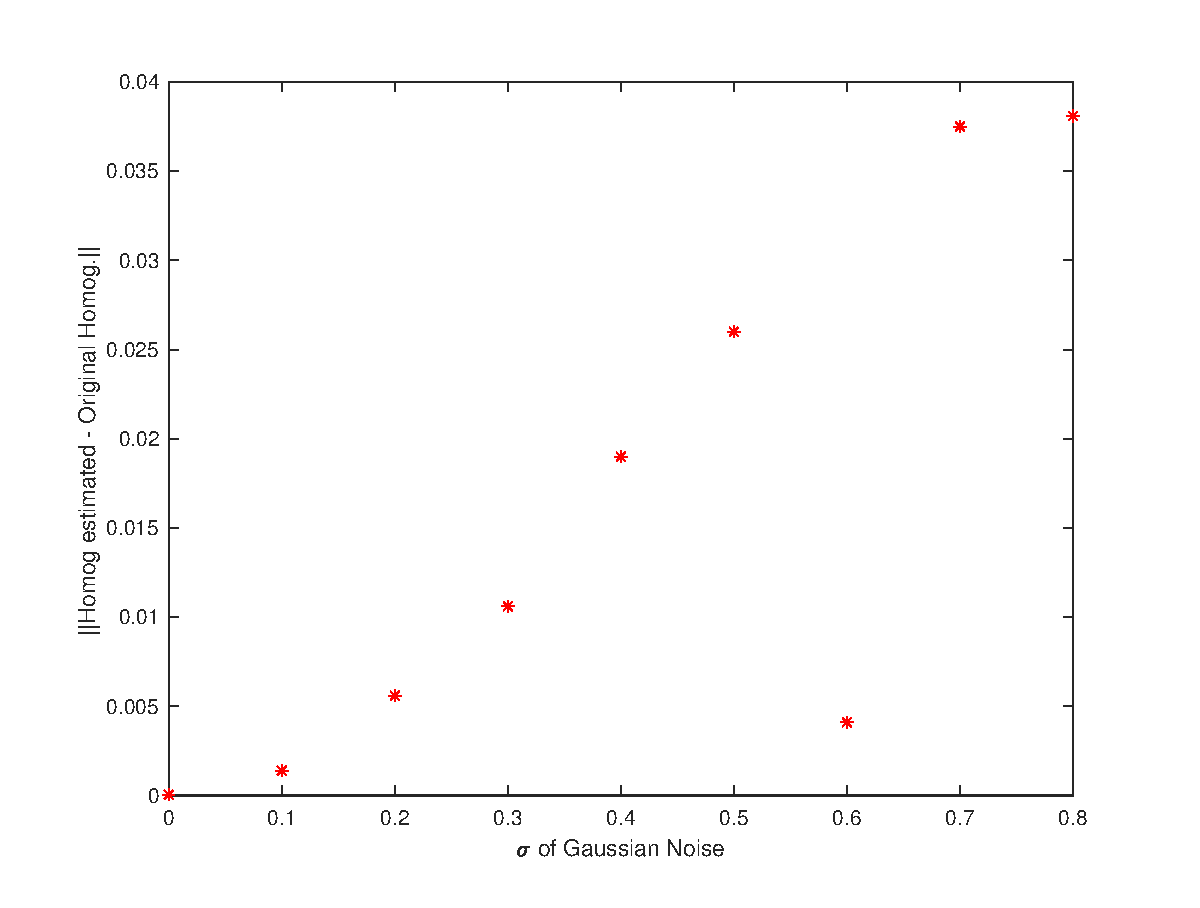
\includegraphics[width = 5.5cm, height=5.5cm]{HomogerrorVsNoiseVariance.eps}
\end{wrapfigure} 
Trend is that more the noise variance i.e. the image pixels of calibration image are more apart from their true values then the worse the error between the Frobenius norm between true Homography matrix and the estimated. Although there is one outlier in the above trend, that is reasonable since we are randomly choosing points each time we run the estimate. So even with the same value of standard deviation and every other parameter, there will be variations in the error values which is why we can explain that as long as the trend is towards worse error with increased variance we can ignore this particular outlier in the above graph.

\subsection{Speed}
Maybe a table of threshold error to quit optim loop and time taken for each value?



\section{Conclusions}
\subsection{Assessment of Data Structures}
\subsection{How would I input real data?}
\subsection{How well did you do?}
Interestingly, results from both these methods were very similar and it was concluded that our forward difference approximation might suffice in this case. This served as a good test for verifying our algorithm for Jacobian.


However, the results we obtained were around a factor of 1000 off from our KMatEstimated. Even so, the optimisation loop was exited (hence the gradient was sufficiently low) which means that there is a strong possibility of the function to be stuck in a local minimum rather than the global minimum. Talk about the convex optimisation leading to global convergence etc. from notes and pawan’s email.


Maybe show 4 tables side by side showing the K-Matrix outputs -1. Original 2. Estimated 3. Optimized 4.using Jacobian and symbolic


\end{document}
